\begin{figure}[!h]
    \centering
    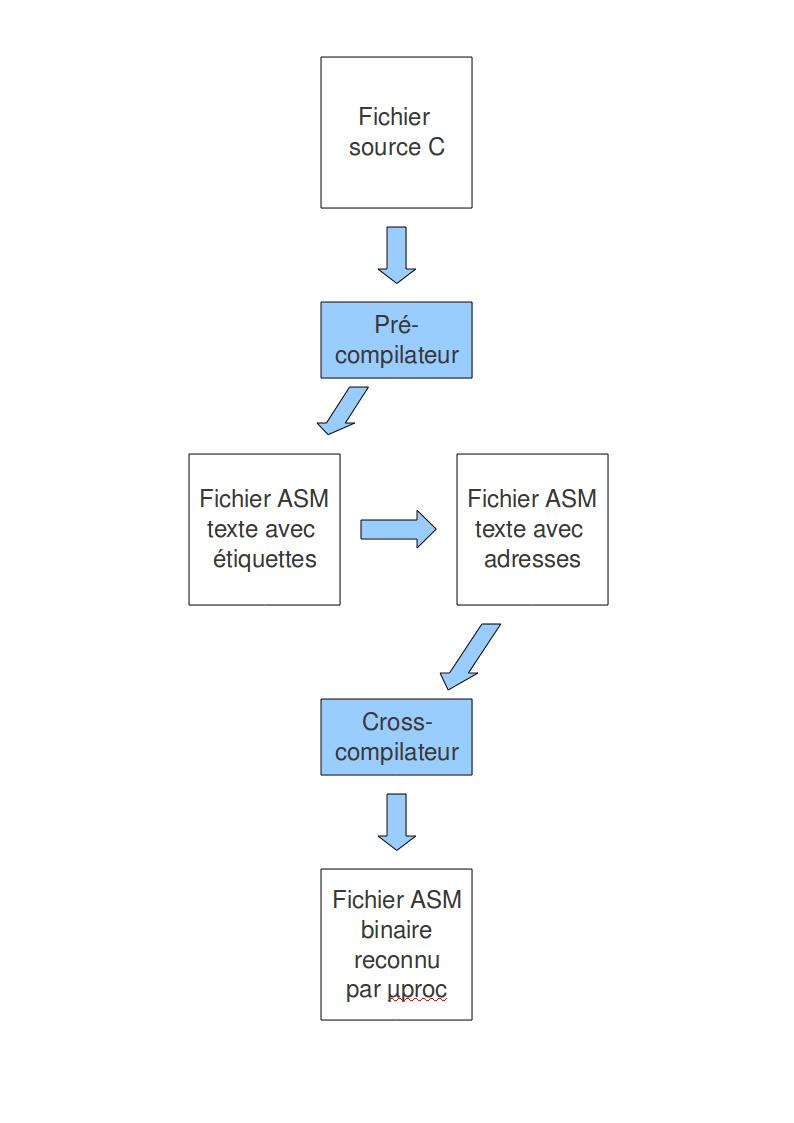
\includegraphics[scale=0.35]{global-compiler.jpg}
    \caption{Schéma de production du binaire exécutable depuis le code source C}
    \label{schema-compilation}
\end{figure}

\subsection{Le pré-compilateur}

\subsubsection{Sa fonction}

Le pré-compilateur a plusieurs fonctions. Tout d’abord, celui-ci fait l’analyse lexicale du fichier source C. Ensuite, l’analyse syntaxique vérifie toutes les règles grammaticales imposées par le langage présentées dans le partie précédente. Si une erreur est détectée, la compilation se poursuit jusqu’à la fin sans générer les fichiers assembleur pour montrer à l’utilisateur l’ensemble de ses erreurs.\\
L’assembleur intermédiaire est généré au fur et à mesure de l’analyse syntaxique. Les instructions prises en compte sont les mêmes que présentées dans le première partie à l'exception du \texttt{STORE} et du \texttt{LOAD} qui sont remplacés pour cette étape par un \texttt{COP}. Aucun registre n’est manipulé, on ne produit que des adresses correspondant à un emplacement dans une pile de valeurs.

\subsubsection{Gestion des variables et des valeurs intermédiaires}

Au stade du pré-compilateur, toutes les valeurs sont imaginées comme stockés dans une pile. Chaque variable ou valeur temporaire a donc une adresse.\\

Prenons l’exemple simple d’une affectation :
\begin{minted}[fontsize=\scriptsize]{c}
  a = a + 1;
\end{minted}

Pour évaluer l’expression de droite :
\begin{enumerate}
\item{Empiler la valeur de \texttt{a} au sommet de la pile}

\item{Empiler la valeur 1}

\item{Additionner les deux valeurs du sommet de pile}

\item{Affecter le résultat à la place du \texttt{a} temporaire}

\item{Mettre à jour la valeur de \texttt{a} avec celle temporaire}
\end{enumerate}

\vspace{10pt}

Pour gérer l’emplacement des variables dans la pile, on utilise la table des symboles. Sa structure est présentée dans la figure \ref{tab:structure-ligne}. Les variables sont insérées dans la table des symboles de la profondeur la plus haute à plus basse (c'est une pile de symboles). Ainsi, si on reprend l’exemple ci-dessous, pour récupérer l’adresse de la variable \texttt{a} de profondeur 2, on cherchera la première variable avec pour identifiant \texttt{a} en partant de la fin de la table des symboles.

\begin{minted}[fontsize=\scriptsize]{c}
  // profondeur 1
  int a = 0;
  
  if (condition) {
    // profondeur 2
    int a = 1;
    
    printf(a); // affiche 1
  }
\end{minted}

\begin{table}[h!]
  \begin{center}
  \begin{tabular}{| l | l | l | l | l |}
    \hline
    Identifiant & Profondeur & Constante & Initialisée & Adresse Pile\\
    \hline
  \end{tabular}
  \end{center}
  {\small
    \textit{Profondeur} permet de gérer la portée d’une variable et savoir si l’on peut déclarer telle variable à telle profondeur.\\
    \textit{Constante} permet de générer une erreur si l’on affecte une valeur à une constante.\\
    \textit{Initialisée} permet d’afficher un warning si la variable est utilisée sans avoir été initialisée.\\
  }
  \caption{Structure d'une ligne de la table des symboles}
  \label{tab:structure-ligne}
\end{table}

\subsubsection{Gestion des sauts}

La gestion des sauts se fait en deux étapes avec génération d'un fichier à la fin de chacune : le premier avec des étiquettes et le second avec des adresses.

\subsubsection*{Les sauts conditionnels}

Lorsqu'on produit le \texttt{JMF} on met une étiquette car on ne connaît pas le nombre d’instructions à sauter. Ce n’est qu’arrivé à la fin du bloc que l’on connaît cette adresse.\\
Pour gérer cela on utilise un tableau d’équivalence étiquette/adresse. À l’indice $n$ correspond l’adresse de l’étiquette \texttt{\$n}.\\
Les imbrications des structures de contrôle compliquent les choses. Il faut raisonner en LIFO : la première étiquette à déterminer est la dernière que l’on va trouver et la dernière étiquette à déterminer est la première que l’on va trouver. Autrement dit, à la fin d’un bloc de structure de contrôle, on remplit la première étiquette non-déterminée de la table en partant de la fin.\\

Voici un exemple de déroulement :
\begin{minted}[fontsize=\scriptsize]{c}
  if(/*...*/) {      //$0 => [ ]
    if(/*...*/){     //$1 => [ ; ]
      // instructions
    }                //$1 => [ ;@1]

    while(/*...*/) { //$2 => [ ; @1 ; ]
      // instructions
    }                //$2 => [ ; @1 ; @2]

    // instruction
  }                  //$0 => [@0 ; @1 ; @2]
\end{minted}

\subsubsection*{Les sauts inconditionnels}

Ils sont utilisés à la fin des blocs \texttt{if} contenant au moins un \texttt{else} après et permettent justement de ne pas aller dans le \texttt{else}, ou bien ils permettent de lancer l’itération suivante dans un \texttt{while}.\\
Pour les \texttt{if} il s’agit de faire un \texttt{JMP} à une étiquette commune. Au début d’un \texttt{if}, on empile dans une autre pile la valeur $i$  de cette étiquette, on consulte cette valeur à chaque fois que l’on insère un \texttt{JMP}. La pile permet là encore de permettre une imbrication de \texttt{if} \texttt{else if} les uns dans les autres. La valeur de l’étiquette est déterminée à la fin du \texttt{if} \texttt{else if}.\\

Voici un exemple de déroulement :
\begin{minted}[fontsize=\scriptsize]{c}
  if (/*...*/) {          // insertion $i : [$i]
    // instructions
    // JUMP $i
  } else if (/*...*/) {
    if (...) {            // insertion $m : [$i,$m]
      // JUMP $m
    } else {

    }
                          // $m : cible du JUMP => adresse $m determinee
                          // depile $m : [$i]
    // JUMP $i
  } else if (/*...*/) {
    // instructions
    // JUMP $i
  } else {
    // intruction
  }
                          // $i : cible des JUMP => adresse de $i determinee
\end{minted}

Pour les \texttt{while}, la technique est un peu différente puisqu’on connait dès le départ l’adresse de l’étiquette mais on ne sait pas où on va placer l’étiquette. On insère donc dans la table des étiquettes une nouvelle étiquette avec son adresse mais en négatif. Arrivé à la fin du \texttt{while}, on recherche la dernière adresse qui est négative et on retrouve l’étiquette associée. Il est ici inutile de mettre une étiquette, on pourrait mettre directement l’adresse puisqu’on la connaît. Mais, cela a été fait pour garder une certaine cohérence du fichier assembleur qui ne sera généré qu’avec des étiquettes.

\subsubsection*{Passage des étiquettes aux adresses :}

Pour finir, à la fin de l’analyse syntaxique on obtient ce fichier assembleur avec des étiquettes mais on connaît toutes les équivalences étiquettes/adresses. On reparse donc le fichier (avec la librairie C) toutes les étiquettes sont remplacées par les bonnes adresses.

\subsection{Le cross-compilateur}

Le cross-compilateur est beaucoup plus simple que le pré-compilateur car celui-ci lui a facilité pas mal le travail.\\

Voici un exemple de fichier qu'il récupère du pré-compilateur.
\begin{lstlisting}
- begin declarations -
- end declarations -
1:	AFC 0xff 1
2:	JMF 0xff 24
- begin declarations -
3:	AFC 0xff 2
4:	NOP
5:	AFC 0xfe 7
6:	NOP
- end declarations -
7:	COP 0xfd 0xff
8:	AFC 0xfc 2
9:	EQU 0xfd 0xfd 0xfc
10:	COP 0xfc 0xff
11:	COP 0xfb 0xfe
12:	AFC 0xfa 7
13:	EQU 0xfb 0xfb 0xfa
14:	AFC 0xfa 1
15:	SUB 0xfb 0xfa 0xfb
16:	MUL 0xfc 0xfc 0xfb
17:	ADD 0xfd 0xfd 0xfc
18:	JMF 0xfd 23
- begin declarations -
19:	AFC 0xfd 0
20:	NOP
- end declarations -
21:	COP 0xfc 0xfd
22:	PRI 0xfc
23:	JMP 1
\end{lstlisting}

Vous pouvez noter la présence de \texttt{NOP} entre les \textit{tokens} \texttt{- begin declarations -} et \texttt{- end declarations -}. Ces deux \textit{tokens} permettent d'interpréter correctement l'instruction \texttt{AFC} suivant le contexte. Si c'est une déclaration de variable, \texttt{AFC} est remplacé par un \texttt{AFC} et un \texttt{STORE}. Un \texttt{AFC} ailleurs reste un \texttt{AFC}. Quant au \texttt{NOP}, il est tout simplement éliminé des intructions. Celui-ci ne servait qu'à garder le décalage pour les sauts du côté du pre-compilateur et n'a plus aucune raison d'être du côté du cross-compilateur.

Le cross-compilateur a deux tâches importantes. La première consiste à distinguer des adresses de variables stockées dans la pile (donc en RAM) de celles correspondant à des registres. La seconde est de traduire les adresses de registres en un numéro de registre.\\
La distinction des adresses de variables dans la RAM est permise du fait de la présences des \textit{tokens} de la zone de déclarations. On sait que l'adresse spécifée au niveau de l'\texttt{AFC} correspond à une variable de la pile. Désormais cette adresse sera présente dans un tableau référençant toutes les adresses de variables en RAM ainsi que leur adresse réelle dans la RAM.\\
Une fois qu'on a fait cette distinction, on peut effectuer en priorité une recherche dans ce tableau pour vérifier si ce n'est pas une adresse dans la RAM. Si c'est le cas, celle-ci est remplacée par sa valeur réelle. Si ce n'est pas une adresse de la pile, il va falloir remplacer cette adresse par un numéro de registre. Un tableau va lui aussi garder la trace des adresses correspondant à un regitre et les registres utilisés. À partir de ces informations, nous allons pouvoir allouer des registres selon nos besoins et les désallouer quand leur contenu n'est plus nécessaire.

\subsection{Le simulateur}

Nous avons codé un simulateur qui lit le fichier binaire généré par le cross-compilateur et exécute les intructions comme le ferait le microprocesseur. Nous pouvons afficher le contenu des registres et de la RAM. Celui-ci nous a permis de debogger efficacement le binaire généré par le cross-compilateur en affinant notre recherche. Nous aurions dû le développer plus tôt car il n'était pas lié au développement du compilateur et nous aurait facilité le développement du cross-compilateur.